\documentclass[serif,UTF8]{ctexart}
\usepackage{amsmath,amssymb,amsfonts}
\usepackage[europeanresistors,americaninductors,americanvoltages,americancurrents,siunitx]{circuitikz}
\usepackage{pgfplots}

\pgfplotsset{width=7cm,compat=1.15}
\usetikzlibrary{datavisualization}
\usetikzlibrary{datavisualization.formats.functions}
\usepgflibrary{arrows.meta}

\renewcommand\CJKfamilydefault{\CJKrmdefault}
\songti\rmfamily

\begin{document}
	切比雪夫滤波器\\
	\begin{tikzpicture}[xscale=1,yscale=1]
		\draw [semithick][-latex'] (-0.25,0) -- (4.5,0) node[right] {$\omega$};
		\draw [semithick][-latex'] (0,-0.25) -- (0,3) node[right] {$|H(j\omega)|$};
		\draw (0,0) node [below left ]{\footnotesize $0$};
		%\draw [dashed](0,1.57) node [left ]{$\frac \pi 2$}--(5,1.57);
		%\draw [dashed](0,-1.57) node [right ]{$-\frac \pi 2$}--(-5,-1.57);
		%\draw [dashed](0.48,0) node [below]{\scriptsize $1.92$}--(0.48,1.57);
		\begin{scope}[xscale=1.5,yscale=2]
			\datavisualization [xy Cartesian,visualize as smooth line]
			data {
			x, y
			0.,1.
			0.025,0.996098
			0.05,0.985105
			0.075,0.968932
			0.1,0.950118
			0.125,0.931241
			0.15,0.914508
			0.175,0.90159
			0.2,0.893624
			0.225,0.89128
			0.25,0.894817
			0.275,0.904091
			0.3,0.91848
			0.325,0.936759
			0.35,0.956951
			0.375,0.976294
			0.4,0.991491
			0.425,0.999388
			0.45,0.997969
			0.475,0.987195
			0.5,0.969125
			0.525,0.947247
			0.55,0.925445
			0.575,0.907193
			0.6,0.895181
			0.625,0.891268
			0.65,0.896505
			0.675,0.911012
			0.7,0.933508
			0.725,0.960478
			0.75,0.985375
			0.775,0.999251
			0.8,0.994531
			0.825,0.970683
			0.85,0.936313
			0.875,0.905204
			0.9,0.891273
			0.925,0.906411
			0.95,0.955479
			0.975,0.999999
			1.,0.891251
			1.025,0.619682
			1.05,0.393748
			1.075,0.255632
			1.1,0.173175
			1.125,0.121938
			1.15,0.0886215
			1.175,0.0660832
			1.2,0.0503269
			1.225,0.0390082
			1.25,0.0306903
			1.275,0.0244588
			1.3,0.0197126
			1.325,0.0160455
			1.35,0.0131762
			1.375,0.0109059
			1.4,0.00909169
			1.425,0.00762876
			1.45,0.0064395
			1.475,0.00546552
			1.5,0.00466241
			1.525,0.00399604
			1.55,0.00343992
			1.575,0.00297331
			1.6,0.00257985
			1.625,0.00224652
			1.65,0.00196288
			1.675,0.00172055
			1.7,0.00151269
			1.725,0.00133376
			1.75,0.0011792
			1.775,0.00104525
			1.8,0.000928797
			1.825,0.000827261
			1.85,0.00073848
			1.875,0.000660645
			1.9,0.00059223
			1.925,0.000531947
			1.95,0.000478706
			1.975,0.000431578
			2.,0.000389771
			};
		\end{scope}
	\end{tikzpicture}

	椭圆滤波器\\
	\begin{tikzpicture}[xscale=1,yscale=1]
		\draw [semithick][-latex'] (-0.25,0) -- (4.5,0) node[right] {$\omega$};
		\draw [semithick][-latex'] (0,-0.25) -- (0,3) node[right] {$|H(j\omega)|$};
		\draw (0,0) node [below left ]{\footnotesize $0$};
		%\draw [dashed](0,1.57) node [left ]{$\frac \pi 2$}--(5,1.57);
		%\draw [dashed](0,-1.57) node [right ]{$-\frac \pi 2$}--(-5,-1.57);
		%\draw [dashed](0.48,0) node [below]{\scriptsize $1.92$}--(0.48,1.57);
		\begin{scope}[xscale=1.5,yscale=2]
			\datavisualization [xy Cartesian,visualize as smooth line]
			data {
			x, y
			0.,1.
			0.025,0.999394
			0.05,0.997593
			0.075,0.994639
			0.1,0.990606
			0.125,0.985589
			0.15,0.979706
			0.175,0.973091
			0.2,0.965892
			0.225,0.958264
			0.25,0.950368
			0.275,0.942368
			0.3,0.934425
			0.325,0.9267
			0.35,0.919352
			0.375,0.912534
			0.4,0.9064
			0.425,0.9011
			0.45,0.896785
			0.475,0.893608
			0.5,0.891723
			0.525,0.891288
			0.55,0.892464
			0.575,0.895414
			0.6,0.900292
			0.625,0.907234
			0.65,0.916328
			0.675,0.927574
			0.7,0.940803
			0.725,0.955558
			0.75,0.970919
			0.775,0.98527
			0.8,0.996091
			0.825,0.999964
			0.85,0.993171
			0.875,0.973296
			0.9,0.941857
			0.925,0.907561
			0.95,0.891515
			0.975,1.0
			1.,0.891251
			1.025,0.147788
			1.05,0.0
			1.075,0.09781
			1.1,0.0966949
			1.125,0.0826258
			1.15,0.0647907
			1.175,0.04662
			1.2,0.029455
			1.225,0.0137821
			1.25,0.000283957
			1.275,0.0127919
			1.3,0.0238583
			1.325,0.0336225
			1.35,0.0422255
			1.375,0.0497998
			1.4,0.0564664
			1.425,0.062333
			1.45,0.0674947
			1.475,0.0720349
			1.5,0.0760266
			1.525,0.0795335
			1.55,0.0826114
			1.575,0.0853088
			1.6,0.0876685
			1.625,0.0897277
			1.65,0.0915192
			1.675,0.093072
			1.7,0.0944113
			1.725,0.0955598
			1.75,0.0965372
			1.775,0.0973613
			1.8,0.0980477
			1.825,0.0986103
			1.85,0.0990617
			1.875,0.0994128
			1.9,0.0996736
			1.925,0.0998532
			1.95,0.0999593
			1.975,0.0999993
			2.,0.0999796
			};
		\end{scope}
	\end{tikzpicture}

	正弦积分函数:\\
	\begin{tikzpicture}[xscale=0.7,yscale=1]
		\draw [semithick][-latex'] (-5,0) -- (5.5,0) node[right] {$x$};
		\draw [semithick][-latex'] (0,-2) -- (0,2.5) node[right] {$Si(x)$};
		\draw (0,0) node [below left ]{\footnotesize $0$};
		\draw [dashed](0,1.57) node [left ]{$\frac \pi 2$}--(5,1.57);
		\draw [dashed](0,-1.57) node [right ]{$-\frac \pi 2$}--(-5,-1.57);
		\draw [dashed](0.48,0) node [below]{\scriptsize $1.92$}--(0.48,1.57);
		\datavisualization [xy Cartesian,visualize as smooth line]
		data {
			x, y
			-5., -1.54824
			-4.875, -1.52863 
			-4.75, -1.51863 
			-4.625,-1.52128 
			-4.5, -1.53661 
			-4.375, -1.56146 
			-4.25, -1.59014 
			-4.125, -1.61563 
			-4., -1.6313 
			-3.875, -1.63258 
			-3.75,-1.61819 
			-3.625, -1.59072
			-3.5, -1.55621 
			-3.375, -1.52291 
			-3.25, -1.49936 
			-3.125, -1.49234 
			-3., -1.50497 
			-2.875,	-1.53571 
			-2.75, -1.57831 
			-2.625, -1.62294 
			-2.5, -1.65835 
			-2.375, -1.67446 
			-2.25, -1.66504 
			-2.125, -1.6296 
			-2.,-1.57419 
			-1.875, -1.51068 
			-1.75, -1.4546 
			-1.625, -1.42179 
			-1.5, -1.42469 
			-1.375, -1.46872 
			-1.25, -1.54993 
			-1.125,-1.65414 
			-1., -1.7582 
			-0.875, -1.83313 
			-0.75, -1.84865 
			-0.625, -1.77852 
			-0.5, -1.60541 
			-0.375, -1.32468 
			-0.25,-0.946083 
			-0.125, -0.493107 
			0., 0. 
			0.125, 0.493107 
			0.25,0.946083 
			0.375, 1.32468 
			0.5, 1.60541 
			0.625,1.77852 
			0.75, 1.84865 
			0.875, 1.83313 
			1., 1.7582 
			1.125,1.65414 
			1.25, 1.54993 
			1.375, 1.46872 
			1.5, 1.42469 
			1.625,1.42179 
			1.75, 1.4546 
			1.875, 1.51068 
			2., 1.57419 
			2.125,1.6296 
			2.25, 1.66504 
			2.375, 1.67446 
			2.5, 1.65835 
			2.625,1.62294 
			2.75, 1.57831 
			2.875, 1.53571 
			3., 1.50497 
			3.125,1.49234 
			3.25, 1.49936 
			3.375, 1.52291 
			3.5, 1.55621 
			3.625,1.59072 
			3.75, 1.61819 
			3.875, 1.63258 
			4., 1.6313 
			4.125,1.61563 
			4.25, 1.59014 
			4.375, 1.56146 
			4.5, 1.53661 
			4.625,1.52128 
			4.75, 1.51863 
			4.875, 1.52863 
			5., 1.54824
		};
	\end{tikzpicture}
	\LaTeX
	单位阶跃函数$\varepsilon (t)$	\\

	\begin{tikzpicture}[scale=1]
					
		\draw [semithick][->] (-0.25,0) -- (3,0) node[right] {$t$};
		\draw [semithick][->] (0,-0.25) -- (0,1.5) node[right] {$\varepsilon(t)$} ;
		\draw [thin](0,1) -- (2.5,1);
		\draw (0,-0.25) node[left] {0} (0,1) node[left] {1};

		\begin{scope}[scale=1,xshift=6cm, yshift=0cm]
			\draw [semithick][->] (-0.25,0) -- (3,0) node[right] {$t$};
			\draw [semithick][->] (0,-0.25) -- (0,1.5) node[right] {$\varepsilon(t)-t_0$} ;
			\draw [thin](0.5,0)--(0.5,1) -- (2.5,1);
			\draw [dashed] (0,1) -- (0.5,1);
			\draw (0,-0.25) node[left] {0} (0,1) node[left] {1} (0.5,0) node[below] {$t_0$};
 		\end{scope}    	

	\end{tikzpicture}	


	单位冲激函数$\delta (t)$\\

	\begin{tikzpicture}[scale=1]
					
		\draw [semithick][->] (-0.8,0) -- (1.2,0) node[right] {$t$};
		\draw [semithick][->] (0,-0.25) -- (0,1.5) node[right] {$\delta(t)$} ;
		\draw [thin][-Stealth] (0,0)--(0,1);
		\draw (0,-0.25) node[left] {0} (0,1) node[left] {$(1)$};

		\begin{scope}[scale=1,xshift=6cm, yshift=0cm]
			\draw [semithick][->] (-0.5,0) -- (1.5,0) node[right] {$t$};
			\draw [semithick][->] (0,-0.25) -- (0,1.5) node[right] {$\delta(t-t_0)$} ;
			\draw [thin][-Stealth] (0.5,0)--(0.5,1);
			\draw (0,-0.25) node[left] {0} (0.5,1) node[right] {$(1)$} (0.5,0) node[below] {$t_0$} ;
 		\end{scope}    	
	\end{tikzpicture}

 	
	\[i(t) = \frac{2}{3}({e^{ - 0.5t}} - {e^{ - 2t}} )\quad i(t) = -\frac{20}{3}({e^{ - 0.5t}} - {e^{ - 2t}} )\]\\

	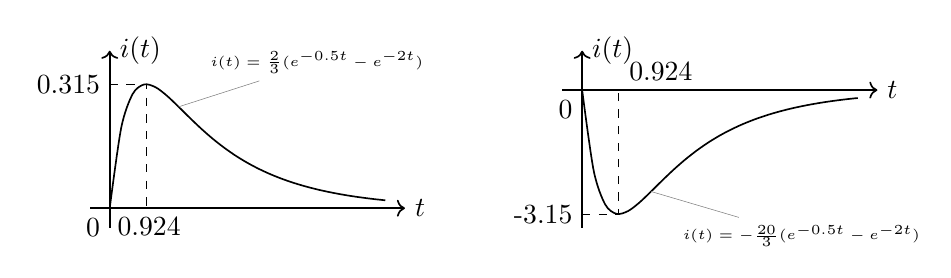
\begin{tikzpicture}[scale=0.5]
	
		\draw [semithick][->] (-0.5,0) -- (7.5,0) node[right] {$t$};
		\draw [semithick][->] (0,-0.5) -- (0,4) node[right] {$i(t)$} ;
		\draw (0,-0.5) node[left] {0} (0,3.15) node[left] {0.315} (1,0) node[below] {0.924};
		\draw [dashed] (0,3.15) -- (0.924,3.15) -- (0.924,0);
		\newcommand\SIGMA{6.66}
		
		\datavisualization [xy Cartesian]
			[
			visualize as smooth line=it,
			it={pin in data={text={\tiny$i(t) = \frac{2}{3}({e^{ - 0.5t}} - {e^{ - 2t}} )$},when=x is 1.5}}
			]
			data [format=function] {
			var x : interval [0:7];
			func y = \SIGMA*(exp(-0.5*\value x)-exp(-2*\value x));
		};

		\begin{scope}[scale=1,xshift=12cm, yshift=3cm]
			\draw [semithick][->] (-0.5,0) -- (7.5,0) node[right] {$t$};
			\draw [semithick][->] (0,-3.5) -- (0,1) node[right] {$i(t)$} ;
			\draw (0,-0.5) node[left] {0} (0,-3.15) node[left] {-3.15} (2,0) node[above] {0.924};
			\draw [dashed] (0,-3.15) -- (0.924,-3.15) -- (0.924,0);
 			%\newcommand\SIGMA{-6.66}
			%\datavisualization [school book axes, visualize as smooth line,x axis={label=$t$},y axis={label=$i(t)~A$}]
        	\datavisualization [xy Cartesian]
				[
				visualize as smooth line=it,
				it={pin in data={text'={\tiny$i(t) = -\frac{20}{3}({e^{ - 0.5t}} - {e^{ - 2t}} )$},when=x is 1.5}}
				]
				data [format=function] {
				var x : interval [0:7];
				func y = -\SIGMA*(exp(-0.5*\value x)-exp(-2*\value x));
			};
 		\end{scope}    
	\end{tikzpicture}


	\[i(t) = \frac{2}{{\sqrt 3 }}{e^{ - \frac{1}{2}t }}\sin \frac{{\sqrt 3 }}{2}t\]

	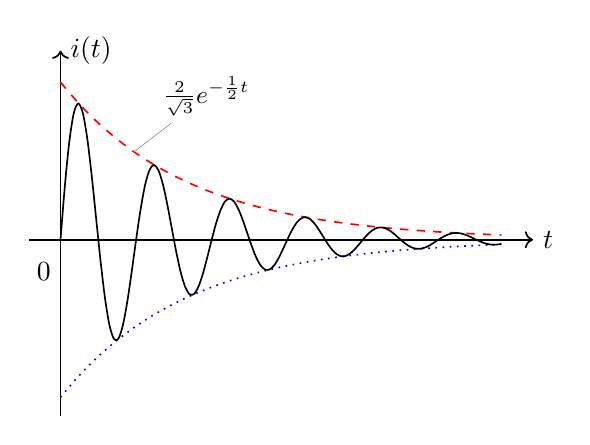
\begin{tikzpicture}[scale=0.8]
		\draw [semithick][->] (-0.5,0) -- (7.5,0) node[right] {$t$};
		\draw [semithick][->] (0,-2.8) -- (0,3) node[right] {$i(t)$} ;
		\draw (0,-0.5) node[left] {0} ;
		%\newcommand\SIGMA{1.1547}
		\datavisualization [xy Cartesian, visualize as smooth line/.list={it,envelope1,envelope2},
					envelope1={pin in data={text={$\frac 2 {\sqrt 3} e^{ -\frac 1 2 t}$},when=x is 1}},
					envelope1={style={dashed,red}},envelope2={style={dotted,blue}}]

			data [set=it,format=function] {
			var x : interval [0:7] samples 100;
			func y = 2.5*(exp(-0.5*\value x)*sin(300*\value x));}

			data [set=envelope1,format=function] {
			var x : interval [0:7];
			func y = 2.5*exp(-0.5*\value x);}

			data [set=envelope2,format=function] {
			var x : interval [0:7];
	  	 	func y = -2.5*exp(-0.5*\value x);	
		};
	\end{tikzpicture}
				
	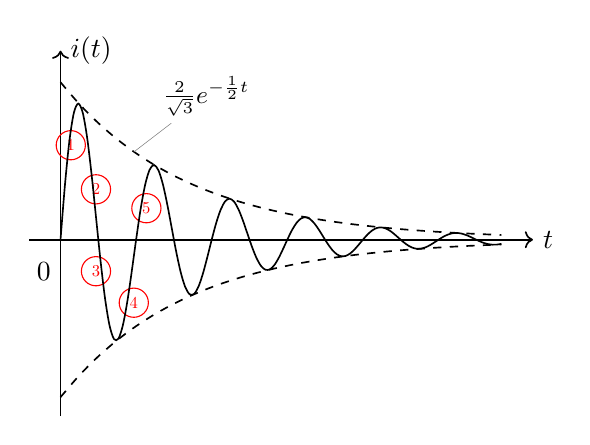
\begin{tikzpicture}[scale=0.8]
		\draw [semithick][->] (-0.5,0) -- (7.5,0) node[right] {$t$};
		\draw [semithick][->] (0,-2.8) -- (0,3) node[right] {$i(t)$} ;
		\draw (0,-0.5) node[left] {0} (0.4,1.5) node[left,color=red,style={circle,draw},scale=0.6] {1}
		(0.8,0.8) node[left,color=red,style={circle,draw},scale=0.6] {2} (0.8,-0.5) node[left,color=red,style={circle,draw},scale=0.6] {3}
		(1.4,-1) node[left,color=red,style={circle,draw},scale=0.6] {4} (1.6,0.5) node[left,color=red,style={circle,draw},scale=0.6] {5};
	
		\datavisualization [xy Cartesian, visualize as smooth line/.list={it,envelope1,envelope2},
					envelope1={pin in data={text={$\frac 2 {\sqrt 3} e^{ -\frac 1 2 t}$},when=x is 1}},
					envelope1={style=dashed},envelope2={style=dashed}]
			data [set=it,format=function] {
			var x : interval [0:7] samples 100;
			func y = 2.5*(exp(-0.5*\value x)*sin(300*\value x));}
			data [set=envelope1,format=function] {
			var x : interval [0:7];
			func y = 2.5*exp(-0.5*\value x);}
			data [set=envelope2, format=function] {
			var x : interval [0:7];
			func y = -2.5*exp(-0.5*\value x);
		};
	\end{tikzpicture}

	抽样函数\\

	\[Sa(t)=\frac{sin(t)}{t}\]
	\begin{tikzpicture}[scale=0.8]
		\draw [semithick][-{Latex}] (-5.5,0) -- (6,0) node[right] {$t$};
		\draw [semithick][-{Latex}] (0,-1) -- (0,4.5) node[right] {$Sa(t)$} ;
		\draw (0,-0.5) node[left] {0} (0,3.5) node[left] {1} (0.8,0) node[below] {$\pi$} (2,0) node[below] {$2\pi$};
						 			
		\datavisualization [xy Cartesian, visualize as smooth line]
			data [format=function] {
			var x : interval [-5:5] samples 200;
			func y = sin(200*\value x)/(\value x);
		};
	\end{tikzpicture}

	正弦函数\\
	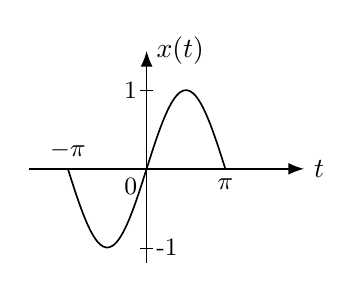
\begin{tikzpicture}
		\draw [semithick][-{Latex}] (-1.5,0) -- (2,0) node[right] {$t$};
		\draw [semithick][-{Latex}] (0,-1.2) -- (0,1.5) node[right] {$x(t)$};
		\draw [thin][-{Bar}] (0,1) node[left] {\small 1};
		\draw [thin][-{Bar}] (0,-1) node[right] {\small -1};
		\draw (-0.2,0) node[below] {\small 0} (-1,0) node[above] {\small $-\pi$} (1,0) node[below] {\small $\pi$};
		\datavisualization [xy Cartesian,visualize as smooth line]
			data [format=function] {
			var x : interval [-1:1] samples 50;
			func y = sin(180*\value x);
		};
	\end{tikzpicture}

	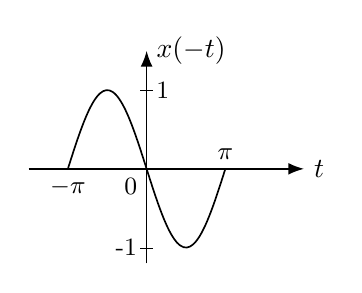
\begin{tikzpicture}
		\draw [semithick][-{Latex}] (-1.5,0) -- (2,0) node[right] {$t$};
		\draw [semithick][-{Latex}] (0,-1.2) -- (0,1.5) node[right] {$x(-t)$};
		\draw [thin][-{Bar}] (0,1) node[right] {\small 1};
		\draw [thin][-{Bar}] (0,-1) node[left] {\small -1};
		\draw (-0.2,0) node[below] {\small 0} (-1,0) node[below] {\small $-\pi$} (1,0) node[above] {\small $\pi$};
		\datavisualization [xy Cartesian,visualize as smooth line]
			data [format=function] {
			var x : interval [-1:1] samples 50;
			func y = -sin(180*\value x);
		};
	\end{tikzpicture}

	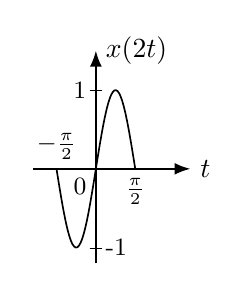
\begin{tikzpicture}
		\draw [semithick][-{Latex}] (-0.8,0) -- (1.2,0) node[right] {$t$};
		\draw [semithick][-{Latex}] (0,-1.2) -- (0,1.5) node[right] {$x(2t)$};
		\draw [thin][-{Bar}] (0,1) node[left] {\small 1};
		\draw [thin][-{Bar}] (0,-1) node[right] {\small -1};
		\draw (-0.2,0) node[below] {\small 0} (-0.5,0) node[above] {\small $-\frac \pi 2$} (0.5,0) node[below] {\small $\frac \pi 2$};
		\datavisualization [xy Cartesian,visualize as smooth line]
			data [format=function] {
			var x : interval [-0.5:0.5] samples 50;
			func y = sin(360*\value x);
		};
	\end{tikzpicture}

	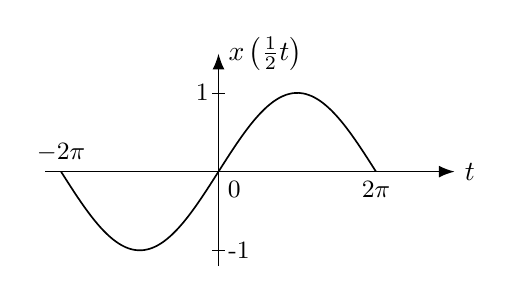
\begin{tikzpicture}
		\draw [semithick][-{Latex}] (-2.2,0) -- (3,0) node[right] {$t$};
		\draw [semithick][-{Latex}] (0,-1.2) -- (0,1.5) node[right] {$x\left(\frac 1 2 t\right)$};
		\draw [thin][-{Bar}] (0,1) node[left] {\small 1};
		\draw [thin][-{Bar}] (0,-1) node[right] {\small -1};
		\draw (0.2,0) node[below] {\small 0} (-2,0) node[above] {\small $-2\pi$} (2,0) node[below] {\small $2\pi$};
		\datavisualization [xy Cartesian,visualize as smooth line]
			data [format=function] {
			var x : interval [-2:2] samples 50;
			func y = sin(90*\value x);
		};
	\end{tikzpicture}

	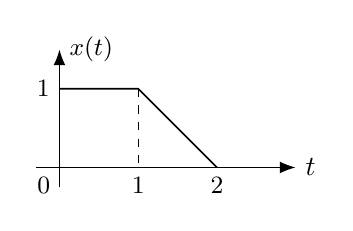
\begin{tikzpicture}
		\draw [semithick][-{Latex}] (-0.3,0) -- (3,0) node[right] {$t$};
		\draw [semithick][-{Latex}] (0,-0.25) -- (0,1.5) node[right] {\small $x(t)$};
		\draw [semithick][-] (0,1)--(1,1)--(2,0) node[below] {\small 2};
		\draw [thin,dashed] (1,1) -- (1,0)  node[below] {\small 1};
		\draw (-0.2,0)  node[below] {\small 0} (0,1)  node[left] {\small 1};
	\end{tikzpicture}
	
	\tikz{
		\draw [semithick][-{Latex}] (-1.3,0) -- (2,0) node[right] {$t$};
		\draw [semithick][-{Latex}] (0,-0.25) -- (0,1.5) node[right] {\small $x(1+t)$};
		\draw [semithick][-] (-1,0)--(-1,1)--(0,1)--(1,0) node[below] {\small 1};
		\draw (-0.2,0)  node[below] {\small 0}  (-1,0)  node[below] {\small -1} (0,1)  node[right] {\small 1}
	}

	\tikz{
		\draw [semithick][-{Latex}] (-1.3,0) -- (2,0) node[right] {$t$};
		\draw [semithick][-{Latex}] (0,-0.25) -- (0,1.5) node[right] {\small $x(1-t)$};
		\draw [semithick][-] (1,0)--(1,1)--(0,1)--(-1,0) node[below] {\small -1};
		\draw (-0.2,0)  node[below] {\small 0}  (1,0)  node[below] {\small 1} (0,1)  node[left] {\small 1}
	}
	\tikz{
		\draw [semithick][-{Latex}] (-1,0) -- (1.6,0) node[right] {$t$};
		\draw [semithick][-{Latex}] (0,-0.25) -- (0,1.5) node[right] {\small $x\left(1-\frac 3 2 t\right)$};
		\draw [semithick][-] (0.67,0)--(0.67,1)--(0,1)--(-0.67,0);
		\draw (-0.2,0)  node[below] {\small 0}  (-0.77,0) node[below] {\small $-\frac 2 3$}
		(0.67,0)  node[below] {\small $\frac 2 3$} (0,1)  node[left] {\small 1}
	}
	\tikz{
		\draw [semithick][-{Latex}] (0,0) -- (1.2,0) node[right] {\tiny $t$};
		\draw [semithick][-{Latex}] (0,0) -- (0,1.5) node[right] {\tiny $e(t)$};
		\draw [semithick][-] (0,0.8)--(0.3,0.8)--(0.3,0);
		\draw (0,0)  node[below] {\tiny 0} 
	}
	\tikz{
		\draw [semithick][-{Latex}] (0,0) -- (1.2,0) node[right] {\tiny $t$};
		\draw [semithick][-{Latex}] (0,0) -- (0,1.5) node[right] {\tiny $e(t-t_0)$};
		\draw [semithick][-] (0.4,0)--(0.4,0.8)--(0.7,0.8)--(0.7,0);
		\draw (0,0)  node[below] {\tiny 0} (0.4,0) node[below] {\tiny $t_0$}
	}

	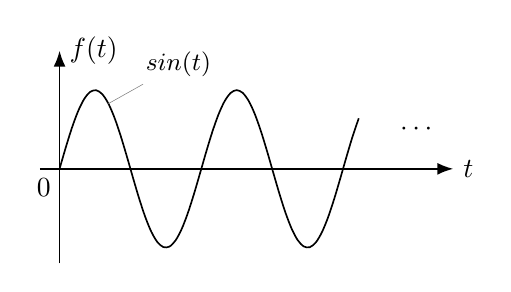
\begin{tikzpicture}
		\draw [semithick][-{Latex}] (-0.25,0) -- (5,0) node[right] {$t$};
		\draw [semithick][-{Latex}] (0,-1.2) -- (0,1.5) node[right] {$f(t)$};
		\draw (-0.2,0) node[below] {0} (4.2,0.5) node[right] {$\cdots$};

		\datavisualization [xy Cartesian,visualize as smooth line=sin ]
			[sin={pin in data={text={$sin(t)$},when=x is 0.6}}]
			data [format=function] {
			var x : interval [0:3.8] samples 50;
			func y = sin(200*\value x);
		};
	\end{tikzpicture}

	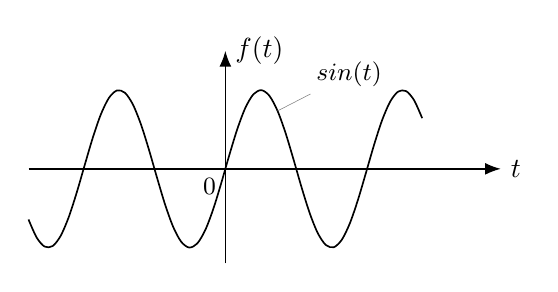
\begin{tikzpicture}
		\draw [semithick][-{Latex}] (-2.5,0) -- (3.5,0) node[right] {$t$};
		\draw [semithick][-{Latex}] (0,-1.2) -- (0,1.5) node[right] {$f(t)$};
		\draw (-0.2,0) node[below] {\small 0};

		\datavisualization [xy Cartesian,visualize as smooth line=sin ]
			[sin={pin in data={text={$sin(t)$},when=x is 0.6}}]
			data [format=function] {
			var x : interval [-2.5:2.5] samples 50;
			func y = sin(200*\value x);
		};
	\end{tikzpicture}

	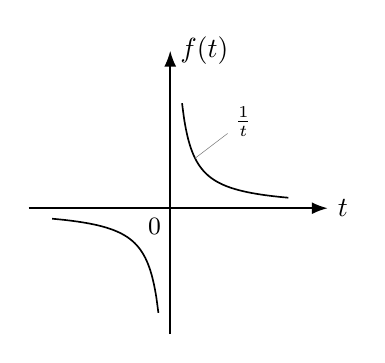
\begin{tikzpicture}
		\draw [semithick][-{Latex}] (-1.8,0) -- (2,0) node[right] {$t$};
		\draw [semithick][-{Latex}] (0,-1.6) -- (0,2) node[right] {$f(t)$};
		\draw (-0.2,0) node[below] {\small 0};

		\datavisualization [xy Cartesian,visualize as smooth line/.list={l1,l2} ]
			[l2={pin in data={text={$\frac 1 t $},when=x is 0.3}}]
			data [set=l1,format=function] {
			var x : interval [-1.5:-0.15] samples 50;
			func y = 0.2/\value x;}
			data [set=l2,format=function] {
			var x : interval [0.15:1.5] samples 50;
			func y = 0.2/\value x;
		};
	\end{tikzpicture}

	\begin{tikzpicture}[scale=1.5]
		\draw [semithick][-{Latex}] (-0.5,0) -- (3,0) node[right] {$t$};
		\draw [semithick][-{Latex}] (0,-0.6) -- (0,1.5) node[right] {$f(t)$};
		\draw [thick][-] (1,-0.368) -- (1,0.368);
		\draw [thin,dashed][-] (0,0.368) -- (1,0.368)  (0,-0.368)--(1,-0.368);
		\draw (-0.1,0) node[below] {\tiny 0} (0,1) node[left] {\tiny $f_0$}
				(0,0.368) node[left] {\tiny $f_1$} (0,-0.368) node[left] {\tiny $f_2$}
				(1.2,0) node[above] {\tiny $t_1$};

		\datavisualization [xy Cartesian,visualize as smooth line/.list={f1,f2}]
			data [set=f1,format=function] {
			var x : interval [0:1] samples 50;
			func y = exp(-\value x);}
			data [set=f2,format=function] {
			var x : interval [1:2.5] samples 50;
			func y =-exp(-2*(\value x-0.5);
		};
	\end{tikzpicture}

	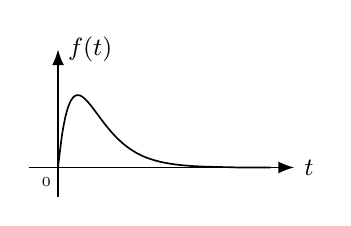
\begin{tikzpicture}[scale=1.5]
		\draw [semithick][-{Latex}] (-0.25,0) -- (2,0) node[right] {\small $t$};
		\draw [semithick][-{Latex}] (0,-0.25) -- (0,1) node[right] {\small $f(t)$};
		\draw (-0.1,0) node[below] {\tiny 0};
		\datavisualization [xy Cartesian,visualize as smooth line]
			data [format=function] {
			var x : interval [0:1.8] samples 50;
			func y =10*(\value x)*exp(-\value x*6);
		};
	\end{tikzpicture}

	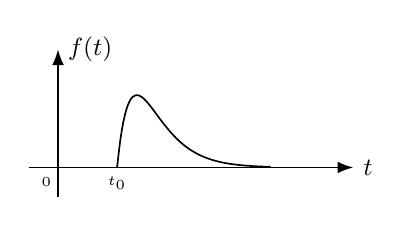
\begin{tikzpicture}[scale=1.5]
		\draw [semithick][-{Latex}] (-0.25,0) -- (2.5,0) node[right] {\small $t$};
		\draw [semithick][-{Latex}] (0,-0.25) -- (0,1) node[right] {\small $f(t)$};
		\draw (-0.1,0) node[below] {\tiny 0} (0.5,0) node[below] {\tiny $t_0$};
		\datavisualization [xy Cartesian,visualize as smooth line]
			data [format=function] {
			var x : interval [0.5:1.8] samples 50;
			func y =10*(\value x-0.5)*exp(-(\value x-0.5)*6);
		};
	\end{tikzpicture}

	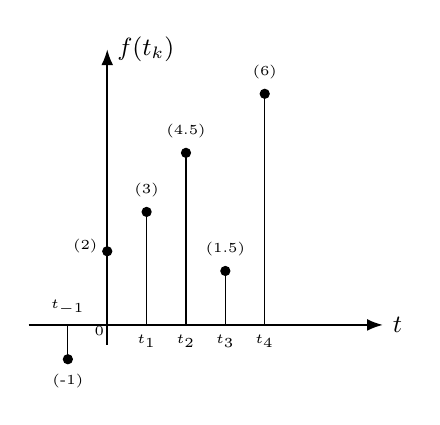
\begin{tikzpicture}[scale=1]
		\draw [semithick][-{Latex}] (-1,0) -- (3.5,0) node[right] {\small $t$};
		\draw [semithick][-{Latex}] (0,-0.25) -- (0,3.5) node[right] {\small $f(t_k)$};
		\draw [thin][-{Circle}] (-0.5,0) -- (-0.5,-0.5) node[below] {\tiny (-1)};
		\draw [thin][-{Circle}] (0,0) -- (0,1) node[left] {\tiny (2)};
		\draw [thin][-{Circle}] (0.5,0) -- (0.5,1.5) node[above] {\tiny (3)};
		\draw [thin][-{Circle}] (1,0) -- (1,2.25) node[above] {\tiny (4.5)};
		\draw [thin][-{Circle}] (1.5,0) -- (1.5,0.75) node[above] {\tiny (1.5)};
		\draw [thin][-{Circle}] (2,0) -- (2,3) node[above] {\tiny (6)};
		\draw (-0.5,0) node[above] {\tiny $t_{-1}$} (-0.1,0.1) node[below] {\tiny 0}
			(0.5,0) node[below] {\tiny $t_1$} (1,0) node[below] {\tiny $t_2$}
			(1.5,0) node[below] {\tiny $t_3$} (2,0) node[below] {\tiny $t_4$}
		;
	\end{tikzpicture}

	\tikz{
		\draw [thick][-{Latex}] (-0.25,0) -- (6,0) node[right] {\small $t$};
		\draw [thick][-{Latex}] (0,-0.25) -- (0,1.6) node[right] {\small $f(t)$};
		\draw[semithick] (4.5,0)--(5,0.333);
		\draw (-0.15,0) node[below] {\small 0} (5,0.6) node[right] {$\cdots$};
		\foreach \x in {0,1.5,3}
			\draw[semithick] (\x,0) -- (\x+1.5,1)--(\x+1.5,0);
	}
	
	\[\displaystyle
		i(t)=e^{-\frac 1 2 t}\left(cos\frac {\sqrt 3} 2 t
		-\frac {\sqrt 3} 3 sin\frac {\sqrt 3} 2 t\right)\varepsilon(t)
	\]

	\[
		u_L(t)=\delta(t)-e^{-\frac 1 2 t}\left(cos\frac {\sqrt 3} 2 t
		+\frac {\sqrt 3} 3 sin\frac {\sqrt 3} 2 t\right)\varepsilon(t)
	\]

	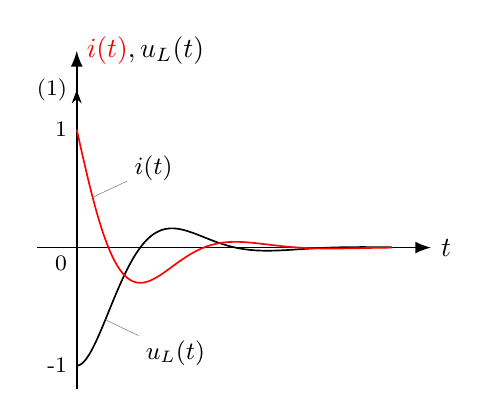
\begin{tikzpicture}[scale=1]
		\draw [semithick][-{Latex}] (-0.5,0) -- (4.5,0) node[right] {$t$};
		\draw [semithick][-{Latex}] (0,-1.8) -- (0,2.5) node[right] {${\color{red}i(t)},u_L(t)$} ;
		\draw [-Stealth](0,-0.2) node[left] {\footnotesize 0} (0,2) node[left] {\footnotesize (1)};
		\draw (0,1.5) node[left] {\footnotesize 1} (0,-1.5) node[left] {\footnotesize -1};
		
		\newcommand\BETA{(sqrt(3)/2)*(180/3.14159)}
		\newcommand\SIGMA{sqrt(3)/3}
		\newcommand\SCALE{3}
		\newcommand\GAIN{1.5}
		\datavisualization [xy Cartesian]
			[visualize as smooth line/.list={it,ul},it={style=red},
			it={pin in data={text={$i(t)$},when=x is 0.2}},ul={pin in data={text'={$u_L(t)$},when=y is -1}}]
			data [set=it,format=function] {
			var x : interval [0:4] samples 100;
			func y =\GAIN*exp(-0.5*\SCALE*\value x)*(cos(\SCALE*\BETA*\value x)-\SIGMA*sin(\SCALE*\BETA*\value x));}
			data [set=ul,format=function] {
			var x : interval [0:4] samples 100;
			func y =-\GAIN*exp(-0.5*\SCALE*\value x)*(cos(\SCALE*\BETA*\value x)+\SIGMA*sin(\SCALE*\BETA*\value x));
		};
	\end{tikzpicture}

	\begin{tikzpicture}
		\draw [semithick][-{Latex}] (-2,0) -- (3,0) node[right] {$x$};
		\draw [semithick][-{Latex}] (0,-0.5) -- (0,3) node[right] {$x^2$} ;
		\datavisualization [xy Cartesian,visualize as smooth line]
		data {
			x, y
			-1.5, 2.25
			-1, 1
			-.5, .25
			0, 0
			.5, .25
			1, 1
			1.5, 2.25
		};
	\end{tikzpicture}
\end{document}